% This is samplepaper.tex, a sample chapter demonstrating the
% LLNCS macro package for Springer Computer Science proceedings;
% Version 2.20 of 2017/10/04
%
\documentclass[runningheads]{llncs}
%
% Used for displaying a sample figure. If possible, figure files should
% be included in EPS format.
\usepackage{float}
\usepackage{graphicx}
\usepackage{hyperref}
\renewcommand\UrlFont{\color{blue}\rmfamily}
\newcommand{\inlinecode}[1]{\texttt{#1}}

\begin{document}
%
\title{Chess-Num - PLOG 2020}
%
%\titlerunning{Abbreviated paper title}
% If the paper title is too long for the running head, you can set
% an abbreviated paper title here
%
\author{João Lucas Silva Martins - 201806436 \and João de Jesus Costa - 201806560}
\author{FEUP-PLOG, Class 3MIEIC03, Group 3}

\institute{Faculty of the engineering of the university of Porto}
\maketitle

\begin{abstract}
This paper is a brief analysis of our solution of the 
\href{https://erich-friedman.github.io/puzzle/chessnum/}{Chess-Num} problem, developed
in the context of the PLOG U.C. The solution is implemented in sicstus prolog using its
finite domain constraints library (clpfd).
TODO copiar conclusao para aqui (conclusões e principais resultados)

%\keywords{First keyword  \and Second keyword \and Another keyword.}
\end{abstract}

\section{Introduction}

In this paper we describe our solution to the \href{https://erich-friedman.github.io/puzzle/chessnum/}{Chess-Num}
problem, which can solve any instance of the puzzle, generate a random solution, and
present the result in a human readable way.
We start by describing the problem, afterwards we explain our implementation, and 
then we analyze the solution/approach.

We weren't able to find any other approaches/references to this problem.

\section{Problem Description}

The Chess-Num problem is a chess-related puzzle in which, given a set of
numbered cells in the chess board, one tries to place the six different chess
pieces (rook, queen, king, bishop, knight pawn) in such a way that the number
of each given cell corresponds to the number of pieces attacking that cell.
The \href{https://erich-friedman.github.io/puzzle/chessnum/}{source} of this
problem has a description of this problem and examples of boards and their solution.
\begin{figure}[H]
  \centering
  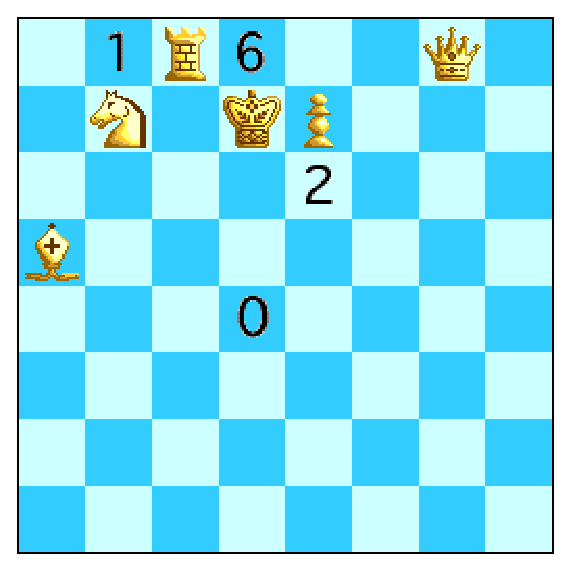
\includegraphics[width=0.5\textwidth]{figures/chessdemo.eps}
  \caption{An example puzzle with four numbered squares and its unique solution.}\label{fig:fig1}
\end{figure}

\section{Approach}
\subsection{Decision Variables}

The decision variables correspond to the coordinate pair of each piece. They are all
within the domain [0, 7] (inclusive). Furthermore, all of these coordinate pairs are
distinct both between each other, as well from the given numbered cells' coordinates.

\subsection{Constraints}

%\subsubsection{All Distinct}
The first restriction placed is applied to the coordinates' pieces. It ensures that all of them
and the chosen cells' coordinates are all different. To achieve this we use the library
predicate \inlinecode{all\_distinct/1} with a list of indices for each coordinate
[X, Y], each index corresponding to $Y * 8 + X$.

%\subsubsection{Value}
The second set of restrictions is applied for each given cell, and it ensures that, for each
one, its value corresponds to number of attacking placed pieces. For this, the \inlinecode{value/3}
predicate is used. It first calculates a boolean value for each piece through the use of the predicate
\inlinecode{value[Piece\_Name]/3}. The calculated value corresponds to 1 if the piece is attacking
the cell and to 0 if it isn't attacking. A sum is then used to verify that the sum of all pieces' values
correspond to the given cell's value.

%\subsubsection{KingValue, KnightValue and PawnValue}
The predicates \inlinecode{valueKing/3, valueKnight/3, valuePawn/3} are straightforward, as
collisions aren't possible with these pieces. Their implementation applies restrictions based
on chess' rules and are as follows: \inlinecode{valueKing/3} yields 1 if the given cell is orthogonally adjacent to
the king; \inlinecode{valueKnight/3} yields 1 if the given cell makes a 'L' pattern
with the knight; \inlinecode{valuePawn/3} yields 1 if the given cell is diagonally and adjacent to
the pawn. If any of these predicates yield 1, constraints are placed to the pieces' coordinates
to ensure that the rules are followed. During the program execution, these constraints may
be too rigid, causing the predicate to fail and backtrack, lifting the placed restrictions and
yielding 0.

%\subsubsection{QueenValue, BishopValue and RookValue}
The predicates \inlinecode{valueQueen/3, valueBishop/3, valueRook/3} behave similarly to
the previous explained predicates when it comes to applying chess rules. The rook can attack
horizontaly or verticaly, the bishop can attack diagonally and the queen can attack horizontaly, verticaly
or diagonally. The main difference is that all of them need also to ensure that no other piece
is placed between their attack path and the given cell.
For this purpose, we use the predicate \inlinecode{others\_is\_not\_between/3}, which calls
\inlinecode{is\_not\_between/3} for each other piece with a given attack path (diagonal, vertical or horizontal)
correspondant to the attacking piece's attack move. \inlinecode{is\_not\_between/3} yields 1 and
restricts the given piece to not be the within attack and can yield 0 through backtrack.
The \inlinecode{others\_is\_not\_between/3} uses this result to verify that all of the members of
the given list aren't in the attacking piece's path. If any other piece blocks the attack path,
this predicate yields 0.

\section{Solution Presentation}

The main (outermost) predicates that allow for a problem/solution visualization
are the \inlinecode{display\_board/1} and the \inlinecode{display\_board/2} predicates.

\subsection{The \inlinecode{display\_board(+NumberedSquares)} predicate}

This predicate will draw a chess board with the given numbered squares coordinates
showing the given values. This is used to show a problem without its solution. It
should be noted that the predicates used to visually represent a solution do so
"on-the-fly". This means that only the input data structures are used instead of
a \textit{game board} structure being generated and displayed.

The call \inlinecode{display\_board([[1, 0]-1, [3, 0]-6, [4, 2]-2, [3, 4]-0]).}
yields the following:
\begin{figure}[H]
  \centering
  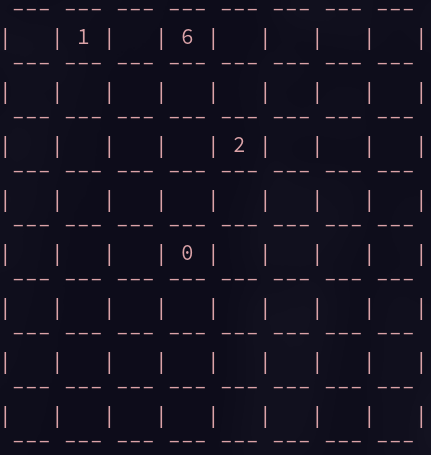
\includegraphics[width=0.5\linewidth]{figures/display_board_1.png}
  \caption{The textual representation of the puzzle show in figure\ref{fig:fig1}
  (without its solution).}\label{fig:fig2}
\end{figure}

\subsection{The \inlinecode{display\_board(+NumberedSquares, +Coords)} predicate}

Similarly to display\_board/1, this predicate will draw a chess board with the given
numbered cells. Along side those, the pieces in the given coordinates will also be
represented. The representation of each piece is as follows: King - \textbf{K},
Queen - \textbf{Q}, Rook - \textbf{R}, Bishop - \textbf{B}, Knight - \textbf{Kn},
and Pawn - \textbf{P}.

The call \inlinecode{display\_board([[1, 0]-1, [3, 0]-6, [4, 2]-2, [3, 4]-0],
[[3, 1], [6, 0], [2, 0], [0, 3], [1, 1], [4, 1]]).} yields the following:
\begin{figure}[H]
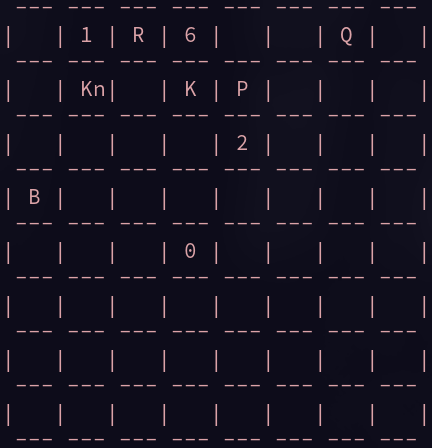
\includegraphics[width=0.5\linewidth]{figures/display_board_2.png}
  \centering
  \caption{The textual representation of the puzzle show in figure\ref{fig:fig1}
  (along side its solution).}\label{fig:fig3}
\end{figure}

\subsection{Innermost display predicates}

// TODO ?

\section{Experiments and Results}
\subsection{Dimensional analysis}
\subsubsection{The impact of the quantity of numbered squares}
The problem in figure~\ref{fig:fig1} is the simplest problem we found with
an unique solution. Our solver finds that solution in about 0.02 seconds.
From the problems in the puzzle's web page, this is the one that is solved
the fastest.

This puzzle has four numbered squares, one of which has the value 6. This
is of note because, we always start constraining the pieces coordinates
in a that they can attack the given numbered square. A numbered square with
value 6 implies that all six pieces are attacking it, thus pruning the
possible coordinates for the pieces by a lot.

We can compare this puzzle to the following which also has a single solution,
but no numbered square with the value 6. It takes about 0.15 seconds to
find the solution. This is significantly higher than the previous one
even though there are the same number of numbered squares.

\begin{figure}[H]
  \centering
  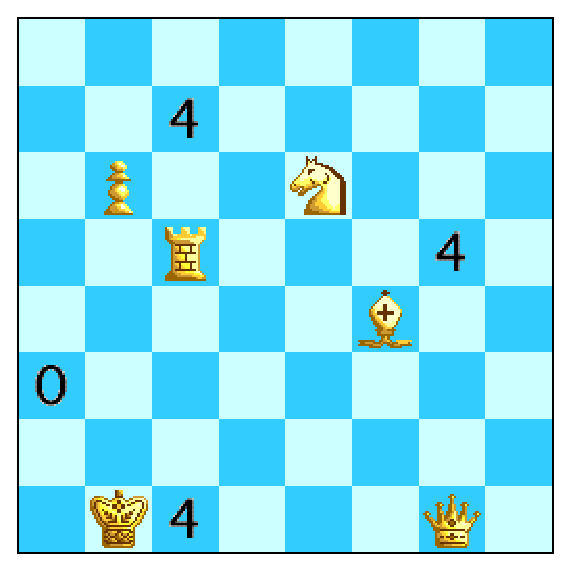
\includegraphics[width=0.5\linewidth]{figures/chess2.eps}
  \caption{A puzzle with four numbered squares and a unique solution.}\label{fig:fig4}
\end{figure}

The more numbered squares the puzzle has, the longer it takes to solve it.

\subsubsection{The special case for the value 0}
As previously stated, our constraints are posted aggressively on the attack
for each for each numbered square. This is very inefficient when the numbered
square we're dealing with has value 0 (no one can attack it). This led us to
create a special case for these numbered squares where we explicitly constraint
all pieces to not attack the numbered square from the get go, instead of
trying to attack it first.

\begin{figure}[H]
  \centering
  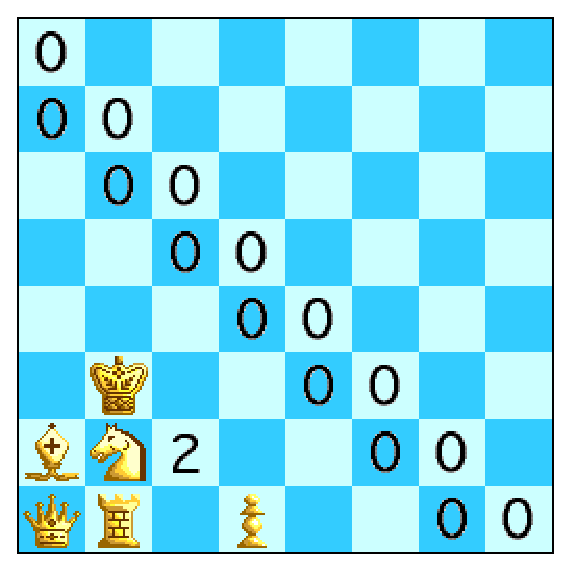
\includegraphics[width=0.5\linewidth]{figures/chess8.eps}
  \caption{A puzzle with four numbered squares and a unique solution.}\label{fig:fig5}
\end{figure}

\subsubsection{The processing order of numbered squares}
When trying new puzzles, we noticed that changing the order of the inputted
numbered squares, thus not changing the problem, but the processing order
of the squares, had an effect on the speed of discovering solutions. This
effect could be has mild has a 0.05 seconds difference or as extreme as some
hours.

The most extreme case we found was following puzzle. This puzzle has a single
solution and the program was tacking hours to find it. By changing the order
the numbered squares are processed, we were able to reduce the processing time
to 7.62 seconds.

\begin{figure}[H]
  \centering
  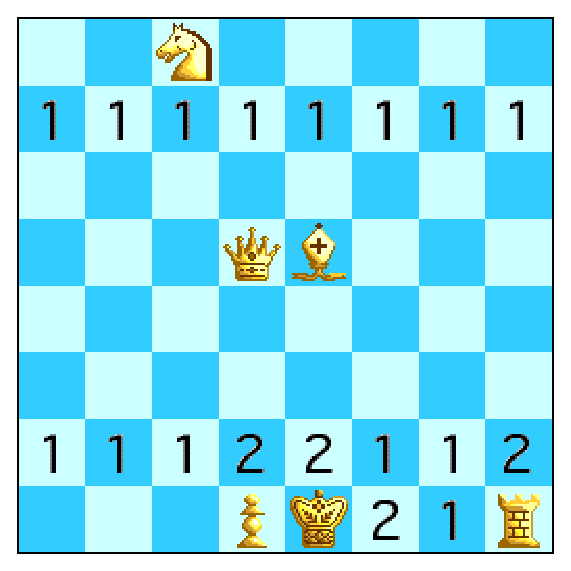
\includegraphics[width=0.5\linewidth]{figures/chess7.eps}
  \caption{A puzzle with four numbered squares and a unique solution.}\label{fig:fig6}
\end{figure}

\section{Conclusions and Future Work}

// TODO site do puzzle + slides do prof + docs do sicstus ?
\begin{thebibliography}{8}
% \bibitem{ref_article1}
% Author, F.: Article title. Journal \textbf{2}(5), 99--110 (2016)

% \bibitem{ref_lncs1}
% Author, F., Author, S.: Title of a proceedings paper. In: Editor,
% F., Editor, S. (eds.) CONFERENCE 2016, LNCS, vol. 9999, pp. 1--13.
% Springer, Heidelberg (2016). \doi{10.10007/1234567890}

% \bibitem{ref_book1}
% Author, F., Author, S., Author, T.: Book title. 2nd edn. Publisher,
% Location (1999)

% \bibitem{ref_proc1}
% Author, A.-B.: Contribution title. In: 9th International Proceedings
% on Proceedings, pp. 1--2. Publisher, Location (2010)

% \bibitem{ref_url1}
% LNCS Homepage, \url{http://www.springer.com/lncs}. Last accessed 4
% Oct 2017
\end{thebibliography}

\section{Annex}

// TODO source code + extra graphs








\end{document}
%
%
%
\section{Template}
\subsection{A Subsection Sample}
Please note that the first paragraph of a section or subsection is
not indented. The first paragraph that follows a table, figure,
equation etc. does not need an indent, either.

Subsequent paragraphs, however, are indented.

\subsubsection{Sample Heading (Third Level)} Only two levels of
headings should be numbered. Lower level headings remain unnumbered;
they are formatted as run-in headings.

\paragraph{Sample Heading (Fourth Level)}
The contribution should contain no more than four levels of
headings. Table~\ref{tab1} gives a summary of all heading levels.

\begin{table}
\caption{Table captions should be placed above the
tables.}\label{tab1}
\begin{tabular}{|l|l|l|}
\hline
Heading level &  Example & Font size and style\\
\hline
Title (centered) &  {\Large\bfseries Lecture Notes} & 14 point, bold\\
1st-level heading &  {\large\bfseries 1 Introduction} & 12 point, bold\\
2nd-level heading & {\bfseries 2.1 Printing Area} & 10 point, bold\\
3rd-level heading & {\bfseries Run-in Heading in Bold.} Text follows & 10 point, bold\\
4th-level heading & {\itshape Lowest Level Heading.} Text follows & 10 point, italic\\
\hline
\end{tabular}
\end{table}


\noindent Displayed equations are centered and set on a separate
line.
\begin{equation}
x + y = z
\end{equation}
Please try to avoid rasterized images for line-art diagrams and
schemas. Whenever possible, use vector graphics instead (see
Fig.~\ref{fig1}).

\begin{figure}
% 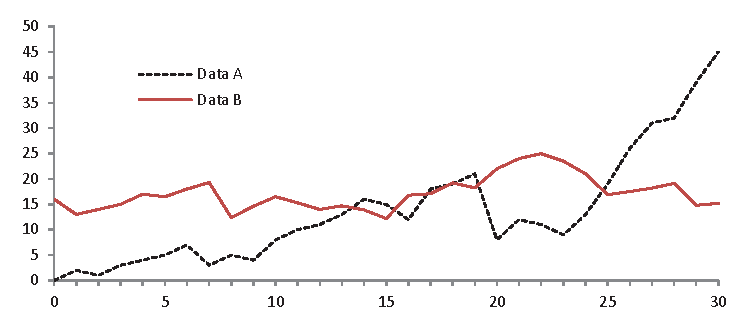
\includegraphics[width=\textwidth]{fig1.eps}
\caption{A figure caption is always placed below the illustration.
Please note that short captions are centered, while long ones are
justified by the macro package automatically.} \label{fig3}
\end{figure}

\begin{theorem}
This is a sample theorem. The run-in heading is set in bold, while
the following text appears in italics. Definitions, lemmas,
propositions, and corollaries are styled the same way.
\end{theorem}
%
% the environments 'definition', 'lemma', 'proposition', 'corollary',
% 'remark', and 'example' are defined in the LLNCS documentclass as well.
%
\begin{proof}
Proofs, examples, and remarks have the initial word in italics,
while the following text appears in normal font.
\end{proof}
For citations of references, we prefer the use of square brackets
and consecutive numbers. Citations using labels or the author/year
convention are also acceptable. The following bibliography provides
a sample reference list with entries for journal
articles~\cite{ref_article1}, an LNCS chapter~\cite{ref_lncs1}, a
book~\cite{ref_book1}, proceedings without editors~\cite{ref_proc1},
and a homepage~\cite{ref_url1}. Multiple citations are grouped
\cite{ref_article1,ref_lncs1,ref_book1},
\cite{ref_article1,ref_book1,ref_proc1,ref_url1}.

